\section{DISSP Architecture} 
% 
% \mnote{4.3 describes the overall architecture, ie it provides the components that will realise the
% logical design from 4.2; as you say, this section should be ls onger than 4.2}
% 
This section describes the overall architecture of the DISSP system.
First, it presents the \emph{high-level components} of a system deployment. DISSP is a distributed
system that is designed to be deployed on a large number of nodes. Every system-wide component that
takes part in the processing of a query will be described, emphasising its role within the
system.

After that, we present the \emph{node architecture}, focusing on the internal operations of a
DISSP node. The different components of a processing node are examined, providing details of some of the
implementation choices and the reasoning behind them. In particular, we describe the
network layer that handles inter-node communication, the operator runner that realises the query
semantics, the load-shedder used to manage overload and the statistics manager that collects
information on the system status.
% 
% When a batch of tuples is received by the node is delivered to the right subqueries, it gets
% processed and finally it is forwarded to the next node to continue processing. A description of these
% steps and about the internal components needed will end the section.
% 
% \todo{WRITE LONGER INTRO!!}

%\clearpage
%
% % -------------------   TEMPLATES   --------------------
% \subsection{Compiled Operators and Tuples}
% \label{sec:templates}
% 
% \mnote{Should this go here? Otherwise, where?}
% 
% In our system tuples and operators are implemented as \emph{compiled POJO objects}. This choice was made
% taking performance into consideration, since other options, based for instance on \emph{reflection}, were considered too
% slow and cause of a potential performance bottleneck. To instantiate a custom tuple or operator object,
% based on the query requirements, a text \textit{template} is completed with the information contained in the XML file
% describing the query producing a new .java file, which is then compiled to bytecode by a run-time compiler. 
% 
% \paragraph{XML Query Representation} Queries are submitted to the system using and XML representation. An
% XML query file contains the complete description of the query. It specifies what kind of tuples will be
% processed, providing a description of the \emph{tuple schemas} so that operators are aware of the
% number, type and name of the fields contained in the tuples they process. It also contains the list of operators
% implementing the query semantic. Every operator is represented by an XML block, containing its
% description. Every operator needs to be specialised before it can be used within a query. A generic
% implementation is provided in a \emph{template file}, which acts as a blueprint for the operator, which
% is then finalised with the data included in the XML block, allowing the correct instantiation of the
% operator.
% The information needed to complete an operator templates includes its \emph{name, parameters} and an indication about its \emph{following operator}. Every operator either declares itself as a
% \emph{terminal} operator, by declaring no downstream operators, or as an \emph{intermediate} operator by
% declaring that its output should be fed in input to another operator. This allows the system to
% reconstruct the complete query graph. 
% The information contained in the XML representation is used to generate the complete .java files
% describing theon customised tuples and operator that will be used in the query. This can then be compiled
% and instantiated so that the query can begin processing. 
% 
% \paragraph{Templates} are semi-complete \textrm{.java} files, representing the skeleton of a class. 
% They are used for the efficient instantiation of customised \textit{tuples} and \textit{operators}.
% All tuples share some common characteristics but are differentiated by the number of fields, their names
% and types. The same is true for all operators belonging to the same type. For instance Average operators
% are all equals when it comes to the processing semantic but they differ about the name and type of the
% field to be averaged. So a generic blueprint for these object comes from the generalisation of a specific
% instance, where specific names and types are replaced by some place text tokens called \emph{place
% holders}. Using the information contained in their XML description it is possible to substitute these
% place holders with the correct details, transforming a template into a complete \textrm{.java} ready for
% compilation.
% Place holders are all capital keywords preceded by a dollar sign, in the
% form ``\texttt{\$PLACEHOLDER}''. They are meant to be completed using the information provided in the XML
% file describing the query and the compiled into actual POJO objects with the desired characteristics. For
% this transformation the system employs a \textit{CharSequenceCompiler}, which takes in input a string
% containing the content of a completed \textrm{.template} file and produces an instance of the customised
% object.
% This allows the system to operate always on compiled bytecode, granting the maximum performance of
% execution together with the flexibility of working with customised versions of tuples and operators
% tailored to the specific query requirements.
% \lstset{
%   basicstyle=\ttfamily,
%   columns=fixed,
%   showstringspaces=false,
%   commentstyle=\color{white}\upshape
% }
% 
% \lstdefinelanguage{XML}
% {
%   morestring=[b]",
%   %morestring=[s]{>}{<},
%   morecomment=[s]{<?}{?>},
%   stringstyle=\color{BrickRed},
%   identifierstyle=\color{NavyBlue},
%   keywordstyle=\color{ForestGreen}, 
%   morekeywords={type,name}% list your attributes here
% }
% \noindent\begin{minipage}{\textwidth}
% \begin{lstlisting}[language=XML,label=lst:opxml,caption=XML description of an Average operator]
% 	<operator name="MyAvgCpu" type="Average">
% 	    <next name="MyOutput"/>
% 	    <parameter name="tuple"    value="simpleSchemaONE" />
% 	    <parameter name="field"    value="cpu"/>
% 	    <parameter name="groupby"  value="idx"/>
% 	<operator>
% \end{lstlisting}
% \end{minipage}
% 
% \exblock{Listing~\ref{lst:opxml} shows the XML description of an \emph{Average} operator. In the first
% line the operator is characterized as being an instance of class ``Average'', described in the correspondant
% .template file, and it is given the name of ``MyAvgCpu'. Then there is the declaration of a \emph{next}
% operator, this means that this is not a terminal operator and thus its output should be delivered to a
% single local operator named ``MyOutput''. Next are 3 parameter definitions, in the form $\langle name,
% value \rangle$. The system will look for the ``\$NAME'' placeholder and will replace it with the string
% given by ``value''. Once the substitution has taken place, the .template file becomes a complete .java
% source file and is then compiled by the \emph{CharSequenceCompiler}.}
% 	
% 
% --------------------   SYSTEM   --------------------
\vspace{-10pt}
\subsection{System-level Components}

\begin{figure}[b!]
	\centering
		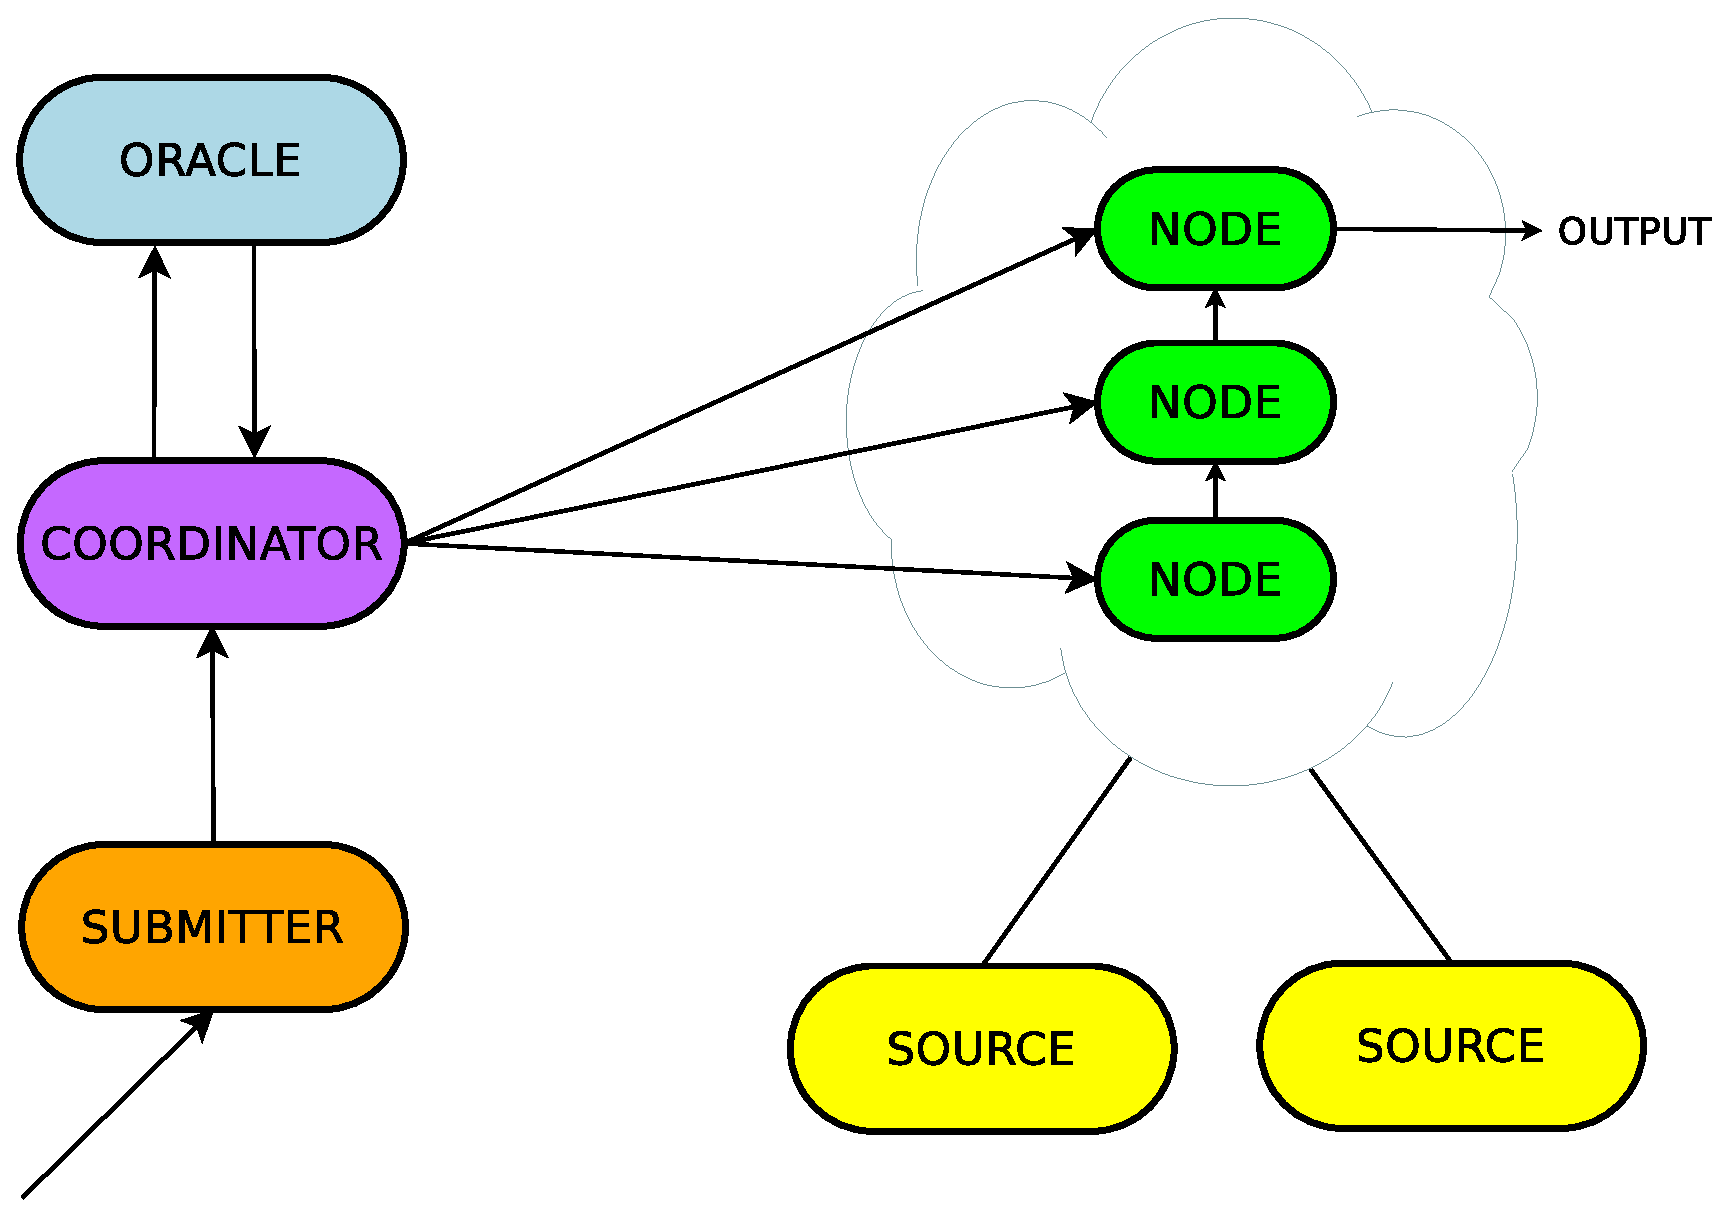
\includegraphics[width=0.6\textwidth]{img/tesi/system_design} 
	\caption{A system level overview of the components in DISSP prototype. }
	\label{fig:sys}
\end{figure}
This section presents the system-level components in the DISSP prototype stream processing system. 
The most important component of all is the \emph{processing node}, a dedicated machine used for the
processing of queries. One or more processing nodes constitute the resource pool onto which all queries
are deployed. Since a query is usually divided into subqueries that are hosted on different processing
nodes, a \emph{coordinator} is deployed for each query. It is hosted on a separate machine and
is in charge of monitoring the status of the query (\ie detecting failed nodes and gathering statistics
about the query performance in terms of achieved quality of processing). \\
A number of data \emph{sources} provide input to the processing nodes. A system-wide \emph{oracle} is
used to obtain a global view of the system. It is aware of all queries and their performance, allowing
to monitor the behaviour of the system as a whole, and is used during query deployment by the
coordinator to provide a list of processing nodes suitable for the deployment of a new query. Finally,
there is also a \emph{submitter}, which provides the user interface to submit one or more queries
for execution. 

Figure~\ref{fig:sys} provides a high-level overview of the DISSP system. Many \emph{processing
nodes} can be deployed in a cloud environment, while some \emph{sources} provide the input data to be
processed.
Queries are deployed through a \emph{submitter}, each having an associated \emph{coordinator} in charge
of its management. An \emph{oracle} oversees the processing of all queries. It gathers information
about their status and performance and also provides the set of nodes onto which new queries
should be deployed.
\vspace{-10pt}
\paragraph*{Processing Node.}
The \emph{processing node} is the component in charge of the execution of operators. It receives tuples through
a network connection. Tuples are converted from their serialised network representation into
concrete instances.
Tuples are then sent to the graph of operators in charge of their processing. After processing by one
node, tuples are sent to the next node to be further processed by the next subquery or are sent to the
output if there is no more processing to be done. Every \emph{processing node} periodically reports to the query \emph{coordinator} about the performance
achieved in terms of quality of processing and to the \emph{oracle} about its throughput and load
condition.
All \emph{processing nodes} are also in charge of performing \emph{load-shedding}, whenever an overload
condition arises. They then make local decisions about which input tuples should be discarded in order to
reduce load. A \mbox{load-shedding} policy designed to achieve \emph{fairness} among all queries running
in the system is the topic of Chapter~\ref{ch:load_shedding}.
% A more detailed description about the internal components and functioning of a \emph{processing node} will be
% provided in Section~\ref{sec:node-arch}.

% \exblock{
% \texttt{java qp.misc.DisspNode <nodeIP> <nodePORT> <oracleIP>}
% 
% This command starts a Processing Node at $\langle nodeIP\rangle$ on port $\langle nodePORT\rangle$.
% The location of the oracle is also passed to the processing node so that it can signal its existence
% and report about its status. After initialisation the processing node remains dormient, until a
% coordinator selects it as a host for the execution of a subquery. 
% } 

\paragraph*{Submitter.} Queries are deployed in the system through the invocation of a
\emph{submitter}.  It receives as input an XML file with the query specifications, including the
\emph{tuple schemas} to be used and the \emph{list of operators}, specifying their type, name, parameters
and connections.
Based on this query description, the \emph{submitter} compiles the individual components of the
query using a runtime compiler, obtaining a set of customised object instantiations, representing the
concrete query in memory. The newly instantiated query is then transformed into a network representation
so that it can be transmitted to a \emph{coordinator}, which is responsible for deployment and
management of the query.
%  In DISSP a \emph{submitter} is designed to be able to start multiple queries at once. It receives a
% file containing a list of XML query files to deploy, with the possibility to specifying beginning and
% ending indexes to start only a certain range of the queries contained in the list. This is particularly
% useful for large deployments and experimental setups.
% Each XML query file is then compiled to bytecode and translated into network format, producing a
% NEW\_QUERY message that is delivered locally.
% This message contains a string representation of the XML query description and of the operators'
% bytecode encoded in Base64.
% The NEW\_QUERY message triggers the creation of a \emph{coordinator}, which handles the deployment and
% management of the new query. In this way a Submitter can instantiate a large number of queries, each
% managed by its coordinator, and can then terminate.

% \exblock{
% \texttt{\\java qp.misc.QuerySubmitter <subIP>  <subPORT> <oracleIP> queryListFile 101 200}
% 
% This command starts a Submitter at $\langle subIP\rangle$ on port $\langle subPORT\rangle$.
% The location of the oracle is also passed to the submitter so that it can be used when instantiating the
% query Coordinators. A \emph{queryListFile} contains a list of paths to XML query
% description files. From this list the Submitter will instantiate only those having index between 101
% and 200 included.
% }
\vspace{-10pt}
\paragraph*{Coordinator.}
Each time a new query is instantiated, a new \emph{coordinator} is created to manage it. This is the
entity in charge of deploying the query on the different \emph{processing nodes}, and all nodes report to
it about their performance. While a submitter can spawn many queries and then terminate, a query is
assigned a \emph{coordinator} that is active for the whole query lifetime. When a query is to be
deployed, the coordinator contacts the \emph{oracle} to receive a list of nodes suitable to host it. 
It then partitions the query graph across a number of processing units and assigns each to a
\emph{processing node}.
After the query was deployed and started, the coordinator acts as a mediator between the
\emph{processing nodes} and the \emph{oracle}, gathering statistics about the query and transferring them
to the \emph{oracle}.
%In DISSP a coordinator is implemented a thread, running on the same machine as the Submitter.
\vspace{-10pt}
\paragraph*{Input Providers.}
An \emph{input provider} is the component that allows input tuples to enter the system, acting as a
collector of external data.
The DISSP system is not concerned with the harvesting of input tuples. 
They are generated elsewhere, for example, by a \emph{sensor network} or through a \emph{social media
environment}.
When the data is available for processing, it is passed to the stream processing system so that queries
can be computed.
The input provider component acts as a \emph{gateway}, at which data is converted to the system
representation and made available to queries for processing. 
Every source can be the entry point for many data sources by employing multiple \emph{InputDevice}
operators.
Each of them connects to an external source, for example, the sink of a sensor network or to the Twitter
firehose.
% In DISSP there are two main kinds of InputDevices operators. The first connects to an external source and 
% then receives tuples as they become available. The other kind instead generate a \emph{synthetic
% workload}, employing a file containing the log of a previous stream of tuples, which are replayed at a
% certain rate. This second option is particularly useful when performing system tests and in experiments
% where different strategies has to be evaluated, for instance comparing the performance of two load
% shedding strategies. A Source can start multiple InputDevice operators at once, so that the same
% component can act as a gateway to multiple real sources.
% A more detailed description about the different types of \emph{input devices} implemented within the
% DISSP system is provided in Section~\ref{sec:input-output}.
% \exblock{
% \texttt{\\java qp.misc.StartSources <sourceIP> <sourcePORT> <oracleIP> sourcesListFile 51 100}
% 
% This command starts a Source at $\langle sourceIP\rangle$ on port $\langle sourcePORT\rangle$. A
% \emph{sourcesListFile} contains a list of paths to XML query description files. Each query is really just
% a SourceInputDevice, that acts as a gateway to the system, through which tuples are input.  From this
% list the Source will instantiate only those having index between 51 and 100 included. Every Source can
% host more than one SourceInputDevice, so that one machine can connect multiple real sources.
% }
\vspace{-10pt}
\paragraph*{Oracle.}
The \emph{oracle} is a system level component that supervises all the processing happening in the
system.
It has two main functions: \emph{monitoring} and \emph{management}. It provides an overview of the
status of all queries so that it is possible to know their achieved quality of processing in real-time. It
also reports the status of all processing nodes, providing information such as their throughput, number
of queries running and their load status. The oracle is also responsible for providing a list of
suitable nodes for deployment of new queries. When a new query is submitted to the
system, its \emph{coordinator} asks the oracle to provide a list of $N$ nodes, which are most suited to
host the new operators.
The \emph{oracle} selects these nodes following a \emph{deployment strategy}, ranking all processing
nodes according to some criteria. For example, it may choose to provide a list of the
\emph{least-loaded} nodes in order to reduce the occurrence of overload conditions, or simply provide a
set of nodes based on a \emph{round-robin} policy.


In the DISSP prototype, the \emph{oracle} is a centralised component and only one instance of it exists
in a system deployment. It is hosted on a dedicated machine and receives messages from
\emph{coordinators}.
% \mnote{Only Coordinators? Terminal Nodes?}
These messages report the quality of processing and other information about the query that they manage, and
also request a list of nodes suitable for deployment when a new query is instantiated.
In addition, the \emph{oracle} provides a web interface so that it is possible to connect to it
using a web browser and access a dashboard with real-time updated information about the system.

In a distributed system, the design choice of a
centralised monitoring entity could seriously hinder scalability. Therefore, the same functionality
could be implemented using an \emph{epidemic} approach~\cite{cyclon}, in which all nodes exchange
gossip messages. A \emph{coordinator} could discover the list
of the least-loaded nodes by participating in gossip communications regarding the load
metric~\cite{vicinity}. A user could monitor the status of a query by participating in gossip
communications with its processing nodes. Even though such a solution would be more scalable, a
centralised approach is simpler to realise.
% --------------------   NODE   --------------------
\subsection{Node Architecture}
\label{sec:node-arch}	
%Every node in the system, at the core, is an instance of the DisspNode class, that gets specialised
% tobecome either a processing node, a source, a submitter or an oracle.
This section describes the internal structure of a DISSP \emph{processing node}.  
A system deployment comprises several processing nodes, hosted at different sites, onto
which queries can be deployed. 
Each node only hosts a partition of a query graph called a \emph{subquery}, while the complete query can
span several nodes. 
Every processing node can host several subqueries belonging to multiple queries.

All inter-node communication passes through the \emph{network layer}, which is responsible for the
handling of \emph{command messages} and \emph{tuples}.
If a command message is received, it triggers an action that is performed directly at the network
level. 
If a \emph{batch of tuples} is received instead, it is passed directly to the \emph{operator runner}
component.
The network layer also provides a \emph{web interface} for remote monitoring.

The \emph{operator runner} delivers the incoming tuples to the appropriate subqueries
and executes the operators.  
It employs a pool of concurrent threads so that multiple operators can execute in
parallel.
Once a subquery has completed its processing on a set of tuples, it sends them to the network layer that
forwards them to the following node to continue processing.

If the incoming input is too large and the node resources are not sufficient to process it completely
without exhausting resources, the \emph{load-shedder} component selects a portion
of it to be discarded in order to overcome the overload condition. 
The selection of the tuples to discard is determined by a \emph{shedding policy}.
Section~\ref{sec:fair-shedding} deals with a strategy trying to shed tuples \emph{fairly} with the
objective of maintaining an equal quality of processing (\ie \sic value) for all queries.

The final important component of a processing node is the \emph{statistic manager}, which is in
charge of collecting statistics about the performance of queries and of the node as a whole. 

\begin{figure}[t!]
	\centering
	\label{fig:node}	
		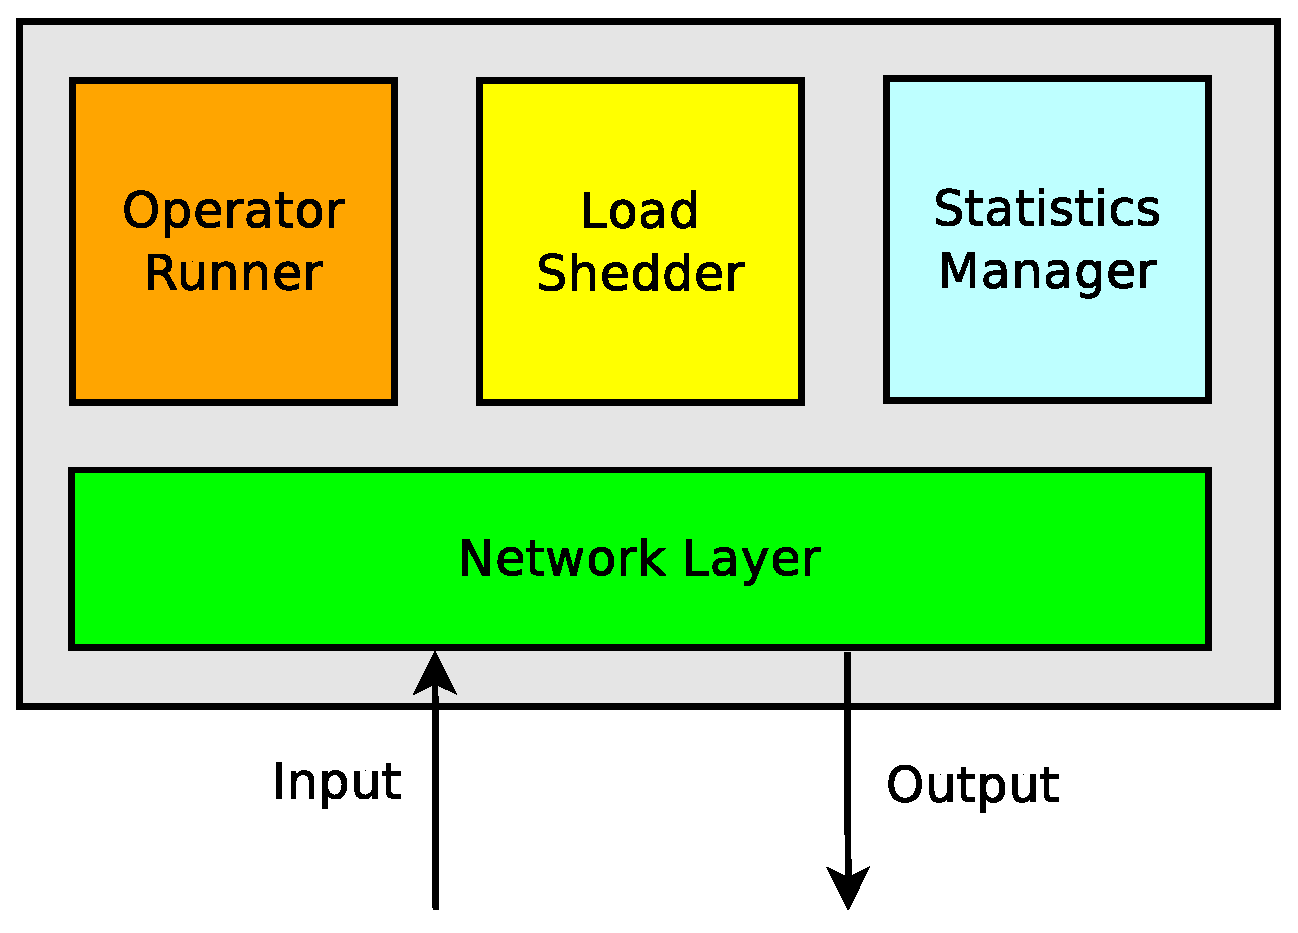
\includegraphics[width=0.5\textwidth]{img/tesi/node} 
		\caption{A high level view of a processing node, with its internal components.}
\end{figure}

\subsection*{Network Layer}  
The network layer is the component that is responsible for all the incoming and outgoing communication
of a processing node. 
It is composed of two threads: the \emph{NioConnector} thread handles all
network communication, and the \emph{RequestHandler} thread interprets the content of the received
messages and acts upon it.
We employ a many-to-one design, in which many remote connections are handled by a single pair
of receiving threads because it offers better scalability. In this way, the
number of active threads in a processing node is constant, thus avoiding the context switch overhead that
a one-to-one threading approach would have.

The \emph{NioConnector} thread acts as a receiver for remote messages as well as a sender for the
outgoing messages. All communication is done through TCP connections, which preserve the integrity of a
network message.
% Using UDP would have increased the chances of a long message being voided by the loss of one of its UDP
% chunks.
The handling of sockets is based on the Java NIO library and is completely asynchronous. This ensures a
low communication overhead and allows one thread to handle all the I/O requests. This many-to-one
design, in which one thread is responsible for all sockets, is preferable to a one-to-one approach,
with one thread for each open socket, due to its simplicity and efficiency. It only employs one CPU
core to handle network communication. Empirical evidence, based on my experience, shows that, even under heavy load and the
presence of a large number of connections, the NioConnector thread never becomes a performance
bottleneck because it only reads or writes network data.
As soon as an incoming message was fully read, it is placed in a queue of pending messages, waiting
to be interpreted by the RequestHandler thread.

The \emph{RequestHandler} thread processes incoming messages. It waits for the
NioConnector thread to place them into its queue and handles them as soon as they become available. All
inter-node communication in the system takes place through \emph{messages}. 
The chosen format for messages is UTF-8 text, with
binary chunks expressed in Base64 encoding. This simple format allows
for easy debugging, even though a binary representation would be more efficient.
The initial task performed by the RequestHandler thread is to interpret the beginning of the message to
categorise it and process it accordingly. A message can be of three kinds: it can be a message
containing \emph{tuples} to be delivered to some subquery for processing; it can contain a \emph{command
message} that triggers the execution of a remote procedure call; or it can be the request to
access the \emph{web interface}.
\vspace{-10pt}
\paragraph{Tuple Handling.}
If a message contains a tuple payload, it is directly passed to the
\emph{operator runner} component without further processing. The content of the message remains in
the network format (\ie it is passed as a string). This follows the principle of \emph{\mbox{lazy
deserialisation}}, which states that the conversion from the network format of tuples should happen as
late as possible. Tuple objects are instantiated only when they are scheduled for processing. Even their
destination (\ie the queries they belong to) is not known until then.
 
The reason for this design choice is that instantiating tuples and determining their destination is a
costly process. In particular, it may be unnecessary to perform it early, when at a later stage the whole
batch may be discarded by the \emph{load-shedder}. Delaying this operation as much as possible ensures
that no resources are wasted to instantiate and route tuples that are never processed.
Our empirical evidence suggests that an early deserialisation also poses a significant processing burden
on the RequestHandler thread, which is unable to handle all messages in a timely fashion under heavy~load.
\vspace{-10pt}
\paragraph{Command Messages.}
A message may also contain a command, triggering a corresponding remote procedure call. This can be
used for communication purposes, reporting information about the status of a node or a query to the
oracle or the query coordinator. Every node, for example, periodically reports its throughput, average
tuple latency and load information to the oracle. It also reports the achieved \sic value
for each query to the respective coordinator, which in turn calculates an aggregated value to be sent to
the oracle. 

Command messages can also be used to obtain information from another node or the oracle. For
example, when a coordinator instantiates a query, it sends a message to the oracle requesting a list
of nodes onto which to deploy the query. During the initial connection stage, when the subqueries running
on different nodes need to connect to each other, it is typical for a node to wait a certain amount
of time for the other node to be ready to accept the connection. A message is used in this situation to
probe the availability of the another node and to wait until it becomes ready.

Another use for command messages is to propagate certain values to a set of nodes. Every node, for
example, needs to be aware of the final \sic value achieved by all queries that are running on it.
By using the global \sic value achieved by every query and comparing it to the local values of the tuples
that it processes, the load-shedder can implement an intelligent load-shedding policy. Therefore, every
coordinator periodically disseminates the global \sic value of its query to all the nodes hosting subqueries.
\vspace{-10pt}
\paragraph{Web Interface.}
The RequestHandler thread is also the gateway to the node's \emph{web interface}. When receiving a
message, it checks if it is an HTTP request and, if so, it replies with a web page containing information
about the current status of the node using the information obtained from the \emph{statistics manager}.
This includes the number of hosted subqueries together with their performance as well as some global
metrics describing the status of the node, such as its average throughput and latency.
When connecting to the oracle, the web interface produces a report about the status of all processing
nodes, together with a summary of the performance achieved by all queries sorted by \sic value. The web
interface of the oracle is useful to monitor the overall performance of the system and to evaluate the
effectiveness of the shedding policy. 

\subsection*{Operator Runner}
After a batch of tuples was received, it is passed to the \emph{operator runner} for processing.
% This is the component in charge of handling the operator processing. 
The operator runner employs a fixed number of threads, each
executing a chain of operators at a time. Bounding the number of processing threads has the
advantage that tuples are processed in the order of arrival and provides more flexibility to the load
shedder, which can freeze the queue of pending jobs and analyse it to make the load-shedding decisions.

The original message, still in its network format, is encapsulated into a \emph{work unit}, a Runnable
class representing a future job to be processed. It is submitted to a ThreadPoolExecutor and placed into
a pending queue until one of the threads in the pool becomes available and executes it. The work unit
contains the logic to deserialise, route and process the tuples contained in the message that it was
assigned. The last operator of the subquery graph is a RemoteSender. It takes the result of
the subquery computation and sends it to the next processing node through the network layer. Once a work
unit has terminated its execution, it frees its execution thread so that a new work unit
can be processed.
\vspace{-10pt}
\paragraph{Thread Pool.}
At the core of the \emph{operator runner} is a \emph{thread pool}, ready to execute work units as
they are submitted. It is a subclass of ThreadPoolExecutor that augments its parent class with the
capability of stopping and resuming execution, which is needed by the load-shedder to inspect the pending
jobs queue. The number of threads is set to be equal to the number of available CPU cores. The pending
jobs queue is a list of work units. As soon as one of the threads in the pool becomes available, it
removes the oldest work unit from the queue and executes it. 

When the system is overloaded, the number of items added to the queue is
larger than the number of items removed, thus making the size of the queue grow. This increases the
latency of processing and eventually leads to an exhaustion of memory. For this reason, the thread
pool is interrupted periodically by the load-shedder, which inspects the pending batches and decides if
there is the need of discarding a certain portion of them in order to overcome overload. The choice
of which ones to discard is part of the shedding policy of the load-shedder.
\vspace{-10pt}
\paragraph{Work Unit.}
A work unit is a container class that has the blueprint to deserialise, route
and process a batch of tuples. Once a work unit is removed from the pending jobs queue and selected
for processing, it is executed by a thread from the pool. 
It starts by deserialising and instantiating the tuples contained in the message received
from the network. It then checks to which query it should be delivered. In case there are multiple
recipients, it creates a copy of itself for each query interested in its payload. After that, it calls
the \texttt{process()} function on the first operator of the query graph. This function takes the
incoming tuples and executes the operator logic, producing one or more batches as output. The work unit
passes these tuples to the next operator and continues processing until it reaches the end of the local subquery
graph. 

A work unit continues processing as long as possible instead of creating a
new work unit for each operator. This permits the system to achieve a higher throughput by reducing
overhead.
Not introducing a new work unit for each operator also guarantees that once a batch of tuples starts
processing, it is not affected by the load-shedder. An approach with one work unit per operator
may result in a batch being processed by a few operators just to be discarded by a later
execution of the load-shedder. If the subquery graph contains an operator with more than one recipient,
such as in a fan-out query, the current work unit continues processing on a single branch, while
creating a new work unit for each of the other operators. 

\subsection*{Load-Shedder}

The \emph{load-shedder} is the component that carries out the \emph{overload management} of a
processing node. When the amount of input tuples rises over a given threshold, the resources available at
the node become insufficient for processing. More tuples are given as input to the node than
what it can process, thus leading to the accumulation of jobs in the pending queue. This causes a growing
increase in latency of the tuples, until the available memory is exhausted.
\vspace{-10pt}
\paragraph{Periodic Evaluation.}
The \emph{CheckOverload} thread periodically runs and evaluates the current load situation of a node.
In the DISSP prototype, a \emph{shedding interval} of 250 milliseconds was chosen, which allows a timely
response to overcome an overload condition while keeping a low performance overhead. Every time the
CheckOverload thread executes, it calculates the number of tuples that the node is able to process
before the next load check.
If this number is greater than the number of tuples currently in the queue waiting to be processed, the
system is not overloaded and no tuples are discarded. If the number of waiting tuples is larger than the
ones that the node manages to process, a certain amount needs to be discarded. 

The system retains a record of its \emph{output rate} (\ie the amount of tuples processed within one
shedding interval). It uses this to calculate the average time needed to process a single tuple called
the \emph{tuple cost}.
Since the shedding interval is
fixed, it is possible to calculate the number of tuples that the system can process before
a new shedding iteration by dividing the \emph{shedding interval} by the \emph{tuple cost}. This
provides the number of tuples \emph{to keep}. Subtracting this number from the \emph{total number of
tuples waiting}, the system obtains the \emph{number of tuples to be discarded}.\\
These numbers depend on many factors. For example, the number of tuples received by a subquery
can be different in a given interval, or the query semantics may produce a variable load
depending on the values contained in the incoming tuples (\ie in the presence of a filter). 
Therefore, the system uses a \emph{sliding window} to average a value for the node's processing capacity
(\ie the forecast number of tuples to process in the next interval) over a few prior iterations thus
reducing the variance of these values. In summary, the periodic cycle followed by the load-shedder is as
follows:
\vspace{-10pt}
%Every time the load-shedder thread executes it follows the same processing steps:
\begin{myenumerate}
  \item Pause the thread pool
  \item Calculate the number of tuples to be discarded
  \item Choose which tuples to shed
  \item Shed the chosen tuples
  \item Resume the thread pool
  \item Update the load metrics 
\end{myenumerate}
\vspace{-10pt}
First, the thread pool has to be stopped in order to obtain the number of tuples that it contains in its
pending queue at this moment. The processing of tuples cannot happen during the execution of the
load-shedder so that it can choose what tuples to discard from a static set. 
After that, it estimates the number of tuples to be discarded, using the logic described in the previous
paragraph.
Once the number of tuples to retain is calculated, the load-shedder can make a decision about
which tuples should be discarded out of the ones available. This choice depends on the \emph{shedding
policy}. A more detailed description of different shedding policies will be given in Chapter~\ref{ch:load_shedding}. 

Then the actual tuples are discarded by removing the corresponding work units from the thread pool queue.
In the DISSP prototype, the granularity of removal is at the level of \emph{batches} because this is the
input/output unit between operators and every work unit is associated with a batch. After performing the
dropping of tuples, the thread pool is restarted and the processing of tuples continues. Before ending
its cycle, the load-shedder calculates the new updated values for the current \emph{tuple cost} and other
internal metrics. Once it finished executing, it calculates the time that it took for processing, called
the \emph{shedding time}, which it subtracts from its fixed interval of execution, called the
\emph{shedding interval}, obtaining the amount of time to sleep before its next execution.

\subsection*{Statistics Manager}
The \emph{statistics manager} is the component responsible for the calculation of the global performance
metrics of a processing node. The metrics gathered by it are used to improve the overall
performance of the system. The load-shedder can exploit its knowledge of the local utility of a
query to implement a fair shedding policy, trying to provide the same processing quality to
all the queries. The oracle, using the information about latency and throughput of nodes, can select the set of
nodes for a new deployment, trying to avoid nodes that are already heavily loaded.

The statistics manager runs periodically, by default once a minute, and calculates a number of
statistics, some of which are logged locally and some are propagated to the coordinator or the
oracle. The following is a list of the most important metrics and their function:

\textbf{Average SIC.} \emph{The average \sic value achieved by queries hosted at this node.}\\
Every subquery is aware of its global \sic value because this value is propagated from the coordinator to
all the processing nodes. This metric is sent to the oracle and can be used during the deployment of
a new query. For a fair deployment strategy, a node already hosting parts of queries
achieving a low global \sic value should not be chosen to host a new subquery. Adding further load
to the node may lead to an overload condition, thus further reducing the processing performance of the
currently running queries. 

\textbf{Average tuple drop.} \emph{The average number of tuples discarded by the node in a chosen time
interval.}\\
This value helps quantifying the amount of overload experienced by a node. It is sent to the
oracle and can be used by a deployment strategy to place a new subquery onto nodes that are not
overloaded or to avoid placing it on a node experiencing already a high tuple loss. 

\textbf{Average throughput.} \emph{The average number of tuples processed by the node in a
chosen time interval.}\\
This value can be used to quantify the spare processing capacity of a node. By
recording the value of this metric when encountering an overload condition, it is possible to have an
indication of the number of tuples per second that this node can process on average without loss. 
This value is sent to the oracle and allows a deployment strategy to choose the least loaded
nodes out of those currently not experiencing overload.\\

\textbf{Average processing latency.} \emph{The average latency in milliseconds for all the hosted
subqueries.}\\
A measure of how much time a tuple spends in this node, from when it is received to when it is delivered
to the next node. This value is sent to the oracle and can be used to discover performance bottlenecks
and to evaluate the quality of the chosen deployment strategy. 
%A good strategy would result in similar latencies at all nodes.

\textbf{Number of running subqueries.} \emph{The number of subqueries running on a node.}\\
This metric can be used to check if the deployment strategy leads to an even
deployment or to a skewed distribution of subqueries. It is sent to the oracle and can also be used to
assess the quality of the chosen deployment strategy.

\textbf{Number of connected subqueries.} \emph{The number of subqueries fully connected.}\\ 
This metric can be used to check the correct deployment of a query.
Every subquery contains at least one incoming network operator (RemoteReceiver) and one outgoing network
operator (RemoteSender). If the query deployment was successful, the number of established connections
should be equal to the number of these operators. A discrepancy indicates that one or more queries are
disconnected either temporary or permanently, which may have been caused by a network partition or a
neighbour node has crashed.
